\chapter{Theory}
\label{theory}

\section{Winter Road Maintenance} % (fold)
\label{sec:snow_plowing}

% \begin{wrapfigure}{o}{0.5\textwidth}
% 	\begin{center}
% 		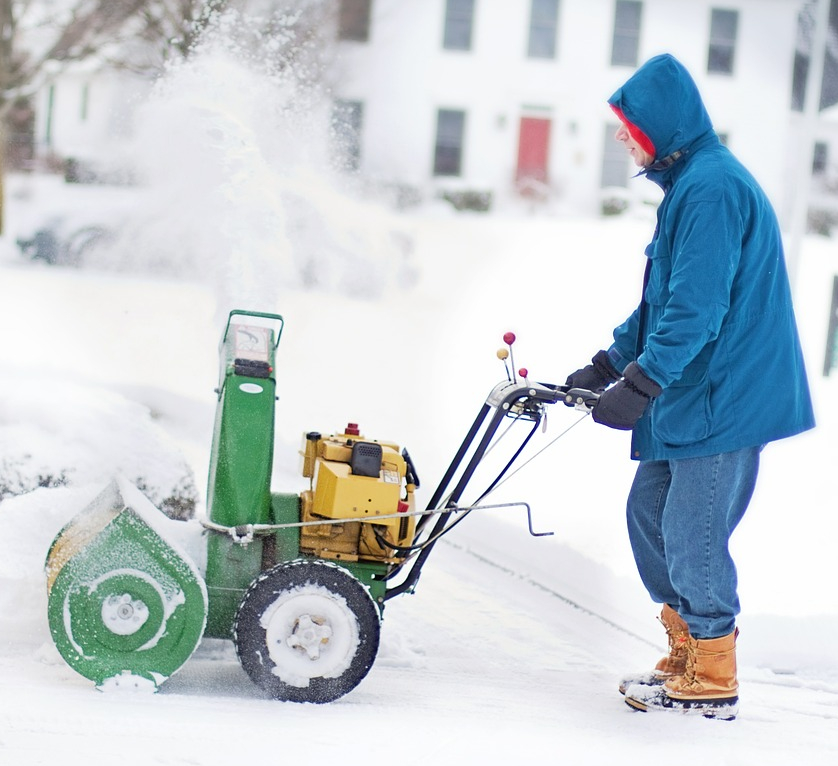
\includegraphics[width=0.5\textwidth]{figures/MachineryIllustrations/pixabay_snow-blower-584380_1280.jpg}
% 	\end{center}
% 	\caption{Snowblower}
% 	\label{fig:snowblower}
% 	% source (2015-06-03T23:38:30Z): http://pixabay.com/en/snow-blower-man-work-winter-snow-584380/
% 	% license: CC0
% \end{wrapfigure}

\begin{wrapfigure}{o}{0.5\textwidth}
	\begin{center}
		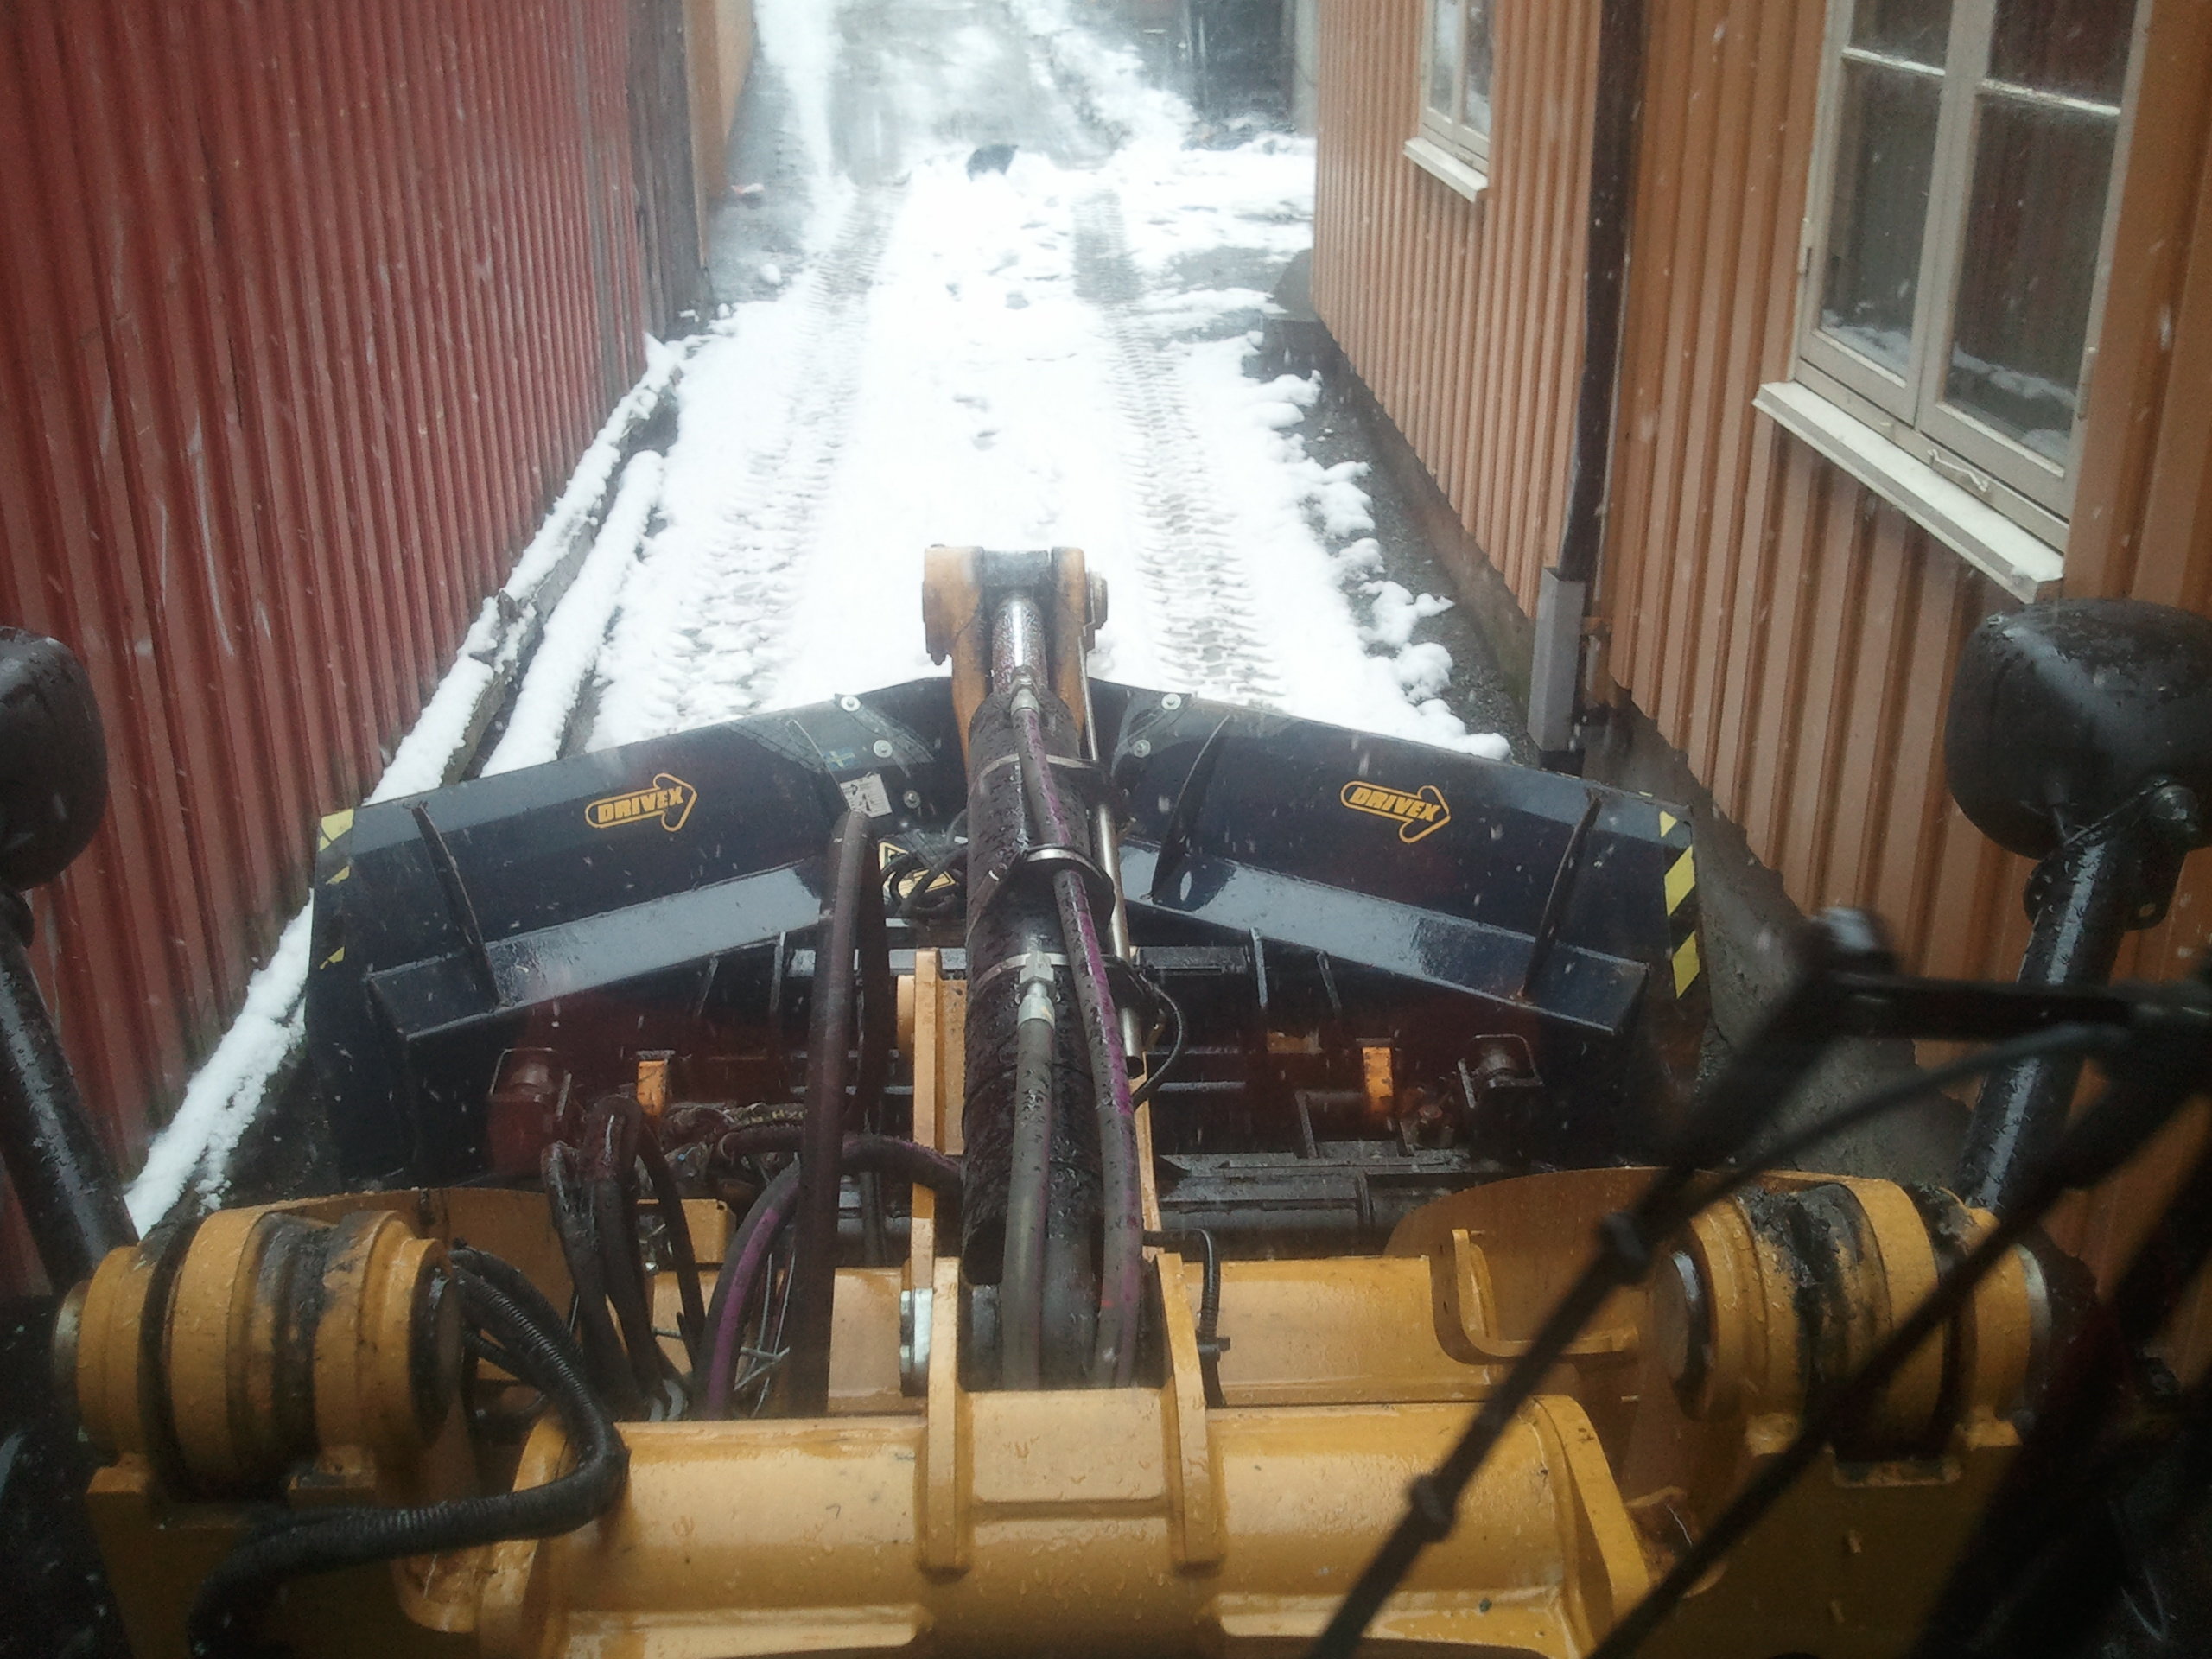
\includegraphics[width=0.5\textwidth]{figures/MachineryIllustrations/snowplow-Kent_Syrstadlokk-2012-04-18.jpg}
	\end{center}
	\caption{Snowplow in a Trondheim alley}
	\label{fig:snowplow_in_alley}
\end{wrapfigure}

In places where the temperature regularly goes below the freezing point of water, winter road maintenance has to be performed. Under such conditions ice can grow on the roads, and they might become blocked by snow. The work done in ensuring that the roads have enough friction to be safe for use by pedestrians and vehicles, and clear enough of snow so that they may pass at all, is what is called winter road maintenance.

The three most common ways of performing winter road maintenance are gritting, salting, and plowing. Gritting describes the act of spreading granular materials such as pebbles or sand on slippery surfaces so that they get more friction. It is often performed on walkways and smaller roads as less resource intensive way to temporarily make it safe for pedestrians and roads with light traffic. In practice sand and combinations of sand and salt are preferred over pebbles when gritting.

Salting is similar to gritting in the sense that the same vehicles and rudimentary process is used to distribute it. However it acts in a different way, and there are other constraints to consider when using it. As opposed to gritting, salting is not done to increase the friction on top of the snow or ice that may be on the road. Instead it is done to melt ice, or ensure that ice does not form in the first place. Thus a desired amount of friction is achieved by keeping the road clean. The main challenge with salting, and the reason that gritting may be preferred over salting in many situations, is that salting on top of a layer of snow has disastrous results. You get a slippery gooey matter that cannot be easily be removed from the road other than by scraping it off. Therefore it is almost always performed as a preventative measure, usually right after a stretch of road has been plowed.

Snow plowing is when snow is cleared by pushing it aside. In daily life various tools are used for clearing snow in this way, such as for an instance general purpose or specialized snow shovels. But for road maintenance vehicle mounted snowplows are the preferred appliance. Although they are not suitable for improving friction arising due to ice, snowplows are great at removing snow that is a direct obstacle to the traffic, and they can improve the friction  by removing densely packed and polished tracks in the snow.

\subsection{Organization of Winter Road Maintenance in Norway and Trondheim} % (fold)
\label{ssub:how_winter_road_maintenance_is_organized_in_norway_and_trondheim}


In Norway the winter road maintenance is a responsibility that is divided between the NPRA, the local municipalities, and the owners of private roads (which are responsible for maintaining their own roads). The NPRA has made two handbooks [håndbok 111 og R610] that specify the constraints on when what kind of winter road maintenance should be performed, and what condition roads should be in after they have been serviced. In [R610] they define 5 classes of winter maintenance standards for roads, as shown in table \ref{tab:wmscfrsbtn}.

\rowcolors{2}{gray!15}{white}
\begin{table}[tbph]
\centering
%ref side 120 i http://www.vegvesen.no/_attachment/61430/binary/964067?fast_title=H%C3%A5ndbok+R610+Standard+for+drift+og+vedlikehold+av+riksveger.pdf
\begin{tabular}{p{0.38\textwidth}p{0.62\textwidth}}
\hline
\textbf{Class Name}                 &  \textbf{Class Description, author's translation}                                                                                    \\ \hline
Winter maintenance class A -- DkA  &  Approved road condition is bare road (dry or wet).                                                                                  \\
Winter maintenance class B -- DkB  &  Approved road condition is bare road (dry or wet), hard snow/ice is permissible outside rut\footnotemark for limited periods.                    \\
Winter maintenance class C -- DkC  &  Approved road condition is bare road (dry or wet) in mild periods and hard snow/ice in cold periods.                                \\
Winter maintenance class D -- DkD  &  Approved road condition is hard snow/ice.                                                                                           \\
Winter maintenance class E -- DkE  &  Approved road condition is hard snow/ice. Friction as low as 0.20 is acceptable. DkE may not be used for national roads.  \\ \hline
\end{tabular}
\caption{Winter maintenance standard classes for roads specified by the NPRA (author's translation)}
\label{tab:wmscfrsbtn}
\end{table}
\footnotetext{track in the road made by the wheels when a lot of vehicles pass}

In addition to being sorted into one of these maintenance classes, each road is also sorted into a functional class by the NPRA. In total the NPRA operates with 10 functional classes depending on the amount of daily traffic, size, etc. However Trondheim municipality only operates with 6 functional classes of roads in their maps. And because the text will mainly be considering winter road maintenance from the municipalitys perspective, the following 6 classes that they have defined (as translated by the author) will be used further in this text:

\begin{itemize}
    \item Riksveg (National road)
    \item Fylkesveg (County road)
    \item Kommunalveg/Hovedveg (Municipal road)
    \item Boliggate (Street)
    \item GS-veg (abbreviation for Gang- og Sykkelvei, translates to Footpaths and Cycle Paths) %https://www.regjeringen.no/en/topics/municipalities-and-regions/by--og-stedsutvikling/framtidensbyer/area-and-transport/footpaths-and-cycle-paths/id547994/
    \item Sykkelfelt (Bicycle lane/path)
\end{itemize}

Out of these the municipality is responsible is responsible for maintaining all, except national and county roads, for which the responsibility falls to the NPRA. As of february the 25th 2015, there are 212 km of municipal roads, 336 km of streets, and 180 km of footpaths and cycle paths that the municipality of Trondheim is responsible for maintaining during the winter (\url{https://www.trondheim.kommune.no/content/1117746169/Vinterdrift-2014-15}, only in Norwegian). To make servicing all these 728 km of roads feasible, they have divided the road network into several smaller zones.

An important factor in deciding the zones is what amount of work can be performed in one trip with the equipment. For gritting the size of each zone may depend on how much sand can be carried before the vehicle has to return to a sand depot to refill. When plowing the size of the zone might be restricted by how fast a vehicle can cover the entirety of it, so that it is returned to the required condition before too much time has passed.

Another important thing that has been considered when creating the zones are what type of equipment is suitable for processing what kind of road. The large municipal roads might be suitable to service with a snowplow truck. Smaller alleys and streets on the other hand are better approached with smaller tractors that can actually fit through them. Therefore when looking at the zones it can be seen that many of them are inside the same area of the map, but containing different roads.

Something the zones in overlapping areas of the map do have in common are the places where the snow is to be stored and disposed of. In the countryside the snow can often be dumped on the side of the road and left there. But in cities, and densely populated areas, it is not so simple. There are various snow depots where the snow is moved for long term storage, and the snow that gets cleared from the city centers proximity is put into the ocean at the harbor. But all of the snow cannot be immediately moved to these locations while the roads are being cleared. Therefore as can be seen on the municipalitys maps, there are marked several locations where snow can be temporarily stored while the work is being performed.

To complete all of this work, the municipality has chosen to handle some of the zones themselves, and set out the other to contractors. The municipality has a lot of the equipment needed for handling the biggest roads, and the intricate situation in the city centre. To operate their equipemnt they use their own drivers. The contractors handling the remaining roads range from individuals that use their own vehicles (typically tractors), to specialized companies with several vehicles and drivers. All of the work is coordinated centrally, by the management at the municipality. They organize both the work carried out by the municipalitys drivers, and that done by the contractors. They set up the schedules for the maintenance work that needs to be done regularly, and call out individual drivers when there has been a weather-incident.

% subsubsection how_winter_road_maintenance_is_organized_in_norway_and_trondheim (end)

Given this outline of how the municipality handles the snow removal part of winter road maintenance, how snow plowing can be modelled and solved needs to be addressed. The next section will explore the models used for similar problems to routing for snow plowing, and what methods have been used to try to find solutions to them.

% section snow_plowing (end)

\section{The Node, Edge, and Arc Rouring Problem}
\label{the_nearp}

In the pre-project leading up to this work we performed a structured literature review (TODO: SOURCE). Our focus was finding whether snow plowing was a known and solved problem, and in case it was, how should one go about trying to solve it. In the following sections we will outline what we found about the classification of the problem, and known approaches.

In our structured literature review we found that the current take on problems like snow plowing has long roots. The simplest possible interpretation is that it is about traversing a graph G=\{N,E\} in a certain way. Which would make it similar to the “Seven bridges of Königsberg Problem”, that is about finding a cycle that traverses the graph and visits all the edges exactly once, and was solved by the Swiss mathematician Leonhard Euler in 1735.

But it was not until more than 200 years later (in 1962) that a graph traversal problem that is more relevant to snow plowing was proposed. The chinese mathematician, and former postman, Mei-Ko Kwan described the problem of finding the shortest trip that visits all the edges in a graph at least once. It is the converse of the Vehicle Routing Problem (VRP), which is about visiting all the nodes of the graph at the lowest possible cost. The problem became known as the Chinese Postman Problem (CPP).

The CPP, if it contains only undirected edges or directed edges (arcs) (G=\{N,E\} or G=\{N,A\}), can be solved in polynomial time. But if it is a mixed graph containing both (G=\{N,E,A\}) it is NP-hard.

Over the following decades several variations on the probem were made to handle specific challenges. We will now briefly define the most known formulations and how they are tied to snow plowing.

The Rural Postman Problem (RPP) arose when one wanted to optimize solutions for when the postman does not have to visit all the edges, but only a subset of them. Which is a situation that is likely to arise in snow plowing, where one for an instance has to service all the roads in a city with a certain amount of traffic, but can pass through the less used roads to move between the ones that have to be plowed.

The Mixed Chinese Postman Problem (MCPP) is the apporach to the CPP where one looks at the problem in a mixed graph (with both arcs and edges). It introduces a relevant constraint when considering practical applications, such as snow plowing, where the underlying graph represents a road network. Not only is it a very natural representation of a road network containing both bi-directional and one way roads, it can also be used to handle cases such as intersections with forbidden turns.

The Hierarchical Chinese Postman Problem (HCPP) came about when one wanted to investigate how solutions would change if one required some edges to be serviced before others. It is a situation that often arises in practice. For an instance in snow plowing one might want to service a more used road before a less used road.

The Windy Postman Problem (WPP) is the attempt at accounting for that an edge can have a different cost each time you pass through it. This is a relevant consideration when snow plowing, because simply passing through a road and plowing it takes a different amount of resources and time, and even passing through a road that has already been plowed and one that has not can have separate costs.

The k-postman Chinese Postman Problem (k-CPP) is the attempt at modeling a scenario where there is a depot node, and k postmen, or one postman that can do k trips of a certain cost. Taking it a step further, the Min-Max k-CPP (MM k-CPP) looks at minimizing the the trip with the maximal cost of the k trips. This is relevant for the snow plowing case where there is a large road network and there is no single vehicle that is capable of service all of it in one go. If implemented correctly it can even be argued that the splitted trips from the k-CPP can be used for sectoring the road network between different contractors.

Now where all these variations on the CPP focus on general graphs, although they arguably can be applied to a broad spectrum of tasks in real world road networks, the Arc Routing Problem (ARP) has also been defined. It is used to describe problems centered around servicing arcs in transport networks. The main difference from the various CPPs tends to be the more vehicle oriented terminology that is used, which makes it somewhat difficult to describe how they relate to one another. It can both be argued that the ARP is a more general version of the CPP with a somewhat different terminology, and that it is a special applied case of the CPP.

What makes it interesting for snow plowing is that in later years the literature dealing with applied routing with the goal of visiting/servicing the arcs and/or edges in a graph has been favoring the ARPs terminology over that of the CPP.

Specially the variation known as the Capacitated Arc Routing Problem (CARP) has been widely studied. It has much in common with the k-CPP, because it deals with the case of having a set of identical vehicles with a limited capacity located at a depot. The task of which is to service the roads in a network in such a way that each road gets serviced by one vehicle once. However, like the k-CPP it suffers from that it is too general to give a good description of complex problems like snow plowing.

This has in turn given rise to definitions that try to include more constraints so that the problems one wants to solve are more accurately described. Within the ARP paradigm the Extended Capacitated Arc Routing Problem (ECARP) has been defined to handle this. It tries to take into account things such as that the problem might be in a mixed graph, the edges/arcs can have a varying cost, special constraints such as u-turns being forbidden in ordinary intersections, a maximum limit on trip lengths, and so on.

The problem definition we found that fits our case best however is the Node Edge and Arc Routing Problem (NEARP). It describes the problem of servicing a subset of the nodes, edges, and arcs in a mixed graph, with a homogeneous set of vehicles. Like in the k-CPP and CARP each vehicle is capacitated in terms of demand it can service (cost it can handle). The elements of the graph that require servicing have a fixed demand, and the all the arcs and edges have a traversal cost while nodes have no traversal cost.

Because it combines the CARP, VRP, and the General Routing Problem, it takes into account all the features of the underlying network we want to use when structuring our graph, such as the assumption of a mixed graph. Another feature that makes it a better model is that it considers both nodes, arcs, and edges as elements of the graph that can need servicing. This makes sense in a snow plowing setting where not only roads and one-way roads, but also intersections need to be plowed.

Now that we have defined what kind of problem we want to solve, we need to look into how it can be solved.


% section the_nearp (end)

% Historical approaches and solutions -> What we gonna use ((M)EA) -> EA -> Fitness -> FLW (basiskomponent) -> Grand tour vs Split som fitness -> Split forklart.

\section{Routing Algorithms} % (fold)
\label{sec:routing_algorithms}

In our structured literature review we came across several methods of solving routing problems. Clearly, the most desirable outcome would be a solution that is known to be optimal. And for the polynomial time cases such as the plain CPP where all the edges have to be serviced by one postman, exact solutions methods exist. But for the NP-hard cases like the CARP, exact solutions quickly become infeasible as problem sizes grow. Some of the best apporaches perform well for problems with up to 7 vehicles, 50 nodes, and 97 edges.

This has lead to efforts in persuing other ways of finding solutions. Some have tried probablistic approaches, but the majority of work has been done on heurisitc methods. Simulated Annealing and Tabu search have been used successfully to give good results. It has been shown that A* can give approximate solutions, but this approach suffers from that there is a signifficant tradeoff between the quality of the solutions it finds, and its capability of processing larger problems within reasonable time.

Other methods that have shown to be robust both in terms of quality of solutions are Ant Colony Optimization (ACO) and Greedy Radnomized Adaptive Search Procedure (GRASP). Both yield solutions of a similar quality as those found by Tabu Search, but ACO outpreforms GRASP on running time.

Lately the most promising results have been given by Evolutionary Algorithms (EA). Genetic Algorithms (GA), a common type of EAs, have been shown to give high quality solutions for large instances of the CARP/NEARP, and and generally outpreform other non-evolutionary methods. A further improvement on GAs has been made by Memetic Algorithms (MA). They have a reasonable running time, and they are capable of finding the highest quality solutions for the larger problem instances.

As such MAs can be considered as the current state of the art apporach to solving the NEARP, which is the reason we chose to base our work with snow plowing in Trondheim on them.

% section routing_algorithms (end)


\section{Evolutionary Algorithms} % (fold)
\label{sec:evolutionary_algorithms}
Now that the reasons for using an EA has been laid out, what EAs are, and how they can be implemented should be discussed. EAs were one of the earliest bio-inspired algorithms, introduced by Alan Turing. The idea is that EAs should mimic the biological processes in evolution, abstracting potential solutions to a population of individuals that have traits which are combined and altered through generations.

A common variant of EAs are GAs. In the paradigm of the GA, at the core of each individual there is a genome. This genome is an alternative representation of a solution to the probem one is trying to solve with the GA that satisfies certain properties.

When there is a new generation, new individuals are made by combining existing members of the population. This is done by taking two or more individuals, and combining their genomes into a new genome, that becomes the foundation for a new individual. A genome must thus be constructed in such a way that it can be merged with another genome in such a way that the output is a valid genome that represents a solution.

Each new genome when created has a chance of undergoing mutation. In practice this often means that one of its components gets an altered value, or two components swap places in the genome, yielding a new altered genome. This ensures that there is always some random variation in the population, making it less prone to becoming stuck in a local optimum.

It must also be possible to convert a genome to a solution of the problem the GA is trying to solve. The solution obtained from a genome is called an individuals phenotype. These phenotypes should take a reasonable time to generate, specially because they are often the foundation for calculating an individuals fitness.

The fitness can then be used to determine whether an optimal solution to the problem has been found. If not, for an instance because it is unknown what a problems global optimal value is, the fitness is often used in determining what individuals are coupled when the nex generation is created, and what combination of pre-existing individuals and new individuals should make up the population at the end of the generation/beginning of the next generation.

To improve on GAs the concept of memeticism can be introduced, turning them into MAs. Memeticism is the term used for describing that individuals can be improved after being generated, mimicing the ability of real life organism in evolutionary systems to learn. In practice this is often done by replacing the mutation step with doing a simple local search, such as hill climbing, to improve the genome.

With the genome being such a central piece in making an EA work, it is natural to let it be the first thing one considers when making a specialized EA for for an instance snow plowing. Our initial approach was to figure out what our genome was to represent. In the case of routing for snow plowing, a solution, and thus what the genome should represent is a route for a snow plow. But what if there, like in the k-CPP and CARP, are several snow plows? Then the genome has to represent a set of trips for each vehicle. Ideally, our genome should be able to represent both these cases.

The solution we found in the literature was to let the genome represent a single circular route, a grand tour of the underlying graph. When dealing with multiple vehicles this tour is splitted into several shorter trips, one for each vehicle. Once the genome and the phenotype it represents is decided, one can begin to look into how the goodness of each individual should be determined, ie. how to calculate the fitness.

% Circular, splittable. 
% Underlying graph -> graph as set -> required elements.
% Giant trip and splittable

% Snow plowing -> Snow plowing genome / phenotype -> How to fitness.

\subsection{Fitness for Snow Plowing} % (fold)
\label{sub:fitness_for_snow_plowing}

There are many things to keep in mind when trying to determine the fitness of a route in a complex operation like snow plowing. In interviews with the municipality and the NPRA, we found some of the most important factors that impact the execution of the plowing, and most likely should affect the goodness of a solution. They are shown in figures \ref{fig:environmental_factors} and \ref{fig:imposed_constraints}.


\begin{figure}[thbp]
\caption{Factors arising from the environment}
\label{fig:environmental_factors}
\begin{description}[noitemsep,nolistsep]
	\item [Amount of traffic.] If there is a lot of traffic, the plows should be expected to move slower.
	\item [Obstacles such as barriers and curbstones.] Some barriers are designed so that they can be forced by studry vehicles such as snow plows moving slowly, while other barriers cannot be passed. Other obstacles such as curbstones can be driven over by some vehicles, while others would be stoped or would damage the curbstone in passing over it.
	\item [Road marking and regulation.] Some places snow plows could be exempt in the marking, allowing them to pass through and service roads other traffic would normally not be allowed to access. Road markings such as forbidden turns should also be taken into consideration when making and working on the graph based on the underlying road network.
	\item [Slope of the road]
	\item [Speed limit]
	\item [Weather.] \begin{description}[noitemsep,nolistsep] \item 
		\item [Quality of the snow.] A lot of wet, heavy, and dense snow will require the vehicles to use more power than a dry, light, and powdery snow.
		\item [Slipperiness of the road.] If there is a lot of ice and the road is very slippery, the vehicles can be expected to work slower.
	\end{description}
	\item [Width of the road.] Affects whether it can be done by a single vehicle or not, and what kind of vehicle is suitable.
\end{description}
\end{figure}

\begin{figure}[thbp]
\caption{Constraints on how the work should be carried out}
\label{fig:imposed_constraints}
\begin{description}[noitemsep,nolistsep]
	\item [Equipment] \begin{description}[noitemsep,nolistsep] \item 
		\item [Amount of vehicles available.]
		\item [Types of vehicles available.]
	\end{description}
	\item [The order the roads are serviced in.] 
	\item [The weather.] The NPRA (addittional source svv booklet) has specified when maintenance should be done, and what shape the road should be in after the maintenance is done.
	\item [The type of road.] Some roads have higher priorities than other roads.
	\item [Where the snow can be stored.] Snow cannot always just be showed to the side out of the road. At times there will be sidewalks or bicycle paths there that should not be blocked by the operation just to have to be services again later. There are pre-defined areas where the snow can be depositioned.
\end{description}
\end{figure}

% When what is needed to calculate the fitness has been obtained, the next step becomes setting up the calculation process.

When one has gained an overview of what variables are needed to find the fitness, the next task becomes setting up the calculation. The format of the benchmarks that we have decided to use as the input format dictates how the values are supplied to the algorithm. Each edge and arc has an associated cost of passing through without doing work, the deadheading cost. Nodes have no deadheading cost. All the factors affecting traversing, simply passing through the graph, should therefore be stored in the deadheading cost.

All the elements in the graph that require servicing, including nodes, also have a servicing cost in addittion to the deadheading cost. The servicing cost is the measure of how much it costs to preform work on the required element. In addittion to the servicing cost, each required element has value for demand. This value is used to indicate how much work needs to be done, in the case of snow plowing it can be interpreted as for an instance the amount of snow that needs to be removed. The capacity of vehicles is expressed as the amount of demand they can service in one trip.

Once the problem has been reduced to a graph G=\{N,E,A\} where each element has these properties, calculating the fitness of a trip becomes a matter of finding the sum of the deadheading and servicing costs in the trip. This can be broken into two sums, the sum of the deadheading costs in the trip, and the sum of the servicing costs. Finding the later is simple, the genome consists of the required elements in the trip, so one just has to iterate over them to find the sum. If the genome encodes a tour of the required elements this sum will remain constant for all tirps.

The next step then becomes finding the costs of going between the required elements in the trip, and the depot node and the first and last element if there is a depot the trip has to start and end in. Because it is a mixed graph the shortest path from one element to another is not neccessairly the shortest path back again, and the shortest path between each required element has to be found with a shortest path algorithm. To find and keep track of these distances we chose to use an all pairs shortest path algorithm and store the output in a distance matrix.

% subsection fitness_for_snow_plowing (end)

\subsection{All Pairs Shortest Path} % (fold)
\label{sub:all_pairs_shortest_path}

\begin{algorithm}[thbp]
\caption{Floyd-Warshall}\label{floyd-warshall-pseudocode}
\begin{algorithmic}[1]

\Procedure{Floyd-Warshall}{Graph}
	\State \textbf{let} $numberOfElements \leftarrow \sum (|N|+|E|+|A|) \in Graph$
	\State \textbf{let} $distances$ be a $numberOfElements \times numberOfElements$ array
	\State \textbf{let} $successors$ be a $numberOfElements \times numberOfElements$ array
	\State \textbf{set} all entries in $distances$ \textbf{to} $\infty$
	\State \textbf{set} all entries in $successors$ \textbf{to} $-1$
	\Statex
	\For{\textbf{each} element $e \in N \cup E \cup A \in Graph$}
		\State $distances[e][e] \leftarrow 0$
		\State $successors[e][e] \leftarrow e$
	\EndFor
	\Statex
	\For{\textbf{each} element $e \in N \cup E \cup A \in Graph$}
		\State \textbf{let} $adjacent \leftarrow $ elements adjacent to $e$ in $Graph$
		\For{\textbf{each} element $e_a \in adjacent$}
			\State $distances[e][e_a] \leftarrow e_a.passThroughCost$
			\State $successors[e][e_a] \leftarrow e_a$
			\State $successors[e_a][e] \leftarrow e$
		\EndFor
	\EndFor
	\Statex
	\For{$k \leftarrow 0$ \textbf{to} $numberOfElements$}
		\For{$i \leftarrow 0$ \textbf{to} $numberOfElements$}
			\For{$j \leftarrow 0$ \textbf{to} $numberOfElements$}
				\If{$distances[i][j] > distances[i][k] + distances[k][j]$}
					\State $distances[i][j] = distances[i][k] + distances[k][j]$
					\State $successors[i][j] = successors[i][k]$
				\EndIf
			\EndFor
		\EndFor
	\EndFor
	\Statex
	\For{\textbf{each} element $(e_i,e_j) \in N \cup E \cup A \in Graph$}
		\If{$e_i \neq e_j$}
			\State $distances[e_j][e_i] \leftarrow distances[e_j][e_i] - e_i.passThroughCost$
		\EndIf
	\EndFor
\EndProcedure

\end{algorithmic}
\end{algorithm}

For verification purposes and being able to show the output on a map should we manage to create a solution that could work with the NPRAs and municipalitys data we also wanted to create a predecessor or successor matrix that would allow us to recreate a trip in its entirety. The two candidates algorithms that would accommodate our needs and be efficient, were Dijkstras algorithm iterated once for each element, or the Floyd Warshall algorithm. We decided to use the Floyd Warshall algorithm because because the code would end up being simpler and therefore more maintainable and easier to modify at a later time than an iterated Dijkstras algorithm.

But before the Floyd Warshall algorithm can be used to find the shortest distance between all the elements from the graph in the genome, it must be decided how the distance between nodes and edges or arcs should be handeled. Usually the resulting shortest path matrix gives the shortest path between nodes. But with how the genome is constructed one will have to know the distance between not only nodes, but also between otehr elements, such as the distance from a required edge to a required arc. A solution to this is to let the algorithm treat every element as it would usually treat nodes, while at the same time treating every element as an arc.

If this is to make sense for using the distance matrix in the fitness calculations, some assumptions have to be made when the matrix is initially set up. Nodes have to add zero cost when moving between elements that are inbound to it or outbound from it. Furthermore, going from a node onto and arc or edge, and conversely going of an arc or edge to a node, should cost zero. However, with these assumptions the Floyd Warshall algorithm should break down giving all paths a cost of zero, because the shortest distance between all neighbors initially is zero.

This can be rectified when initializng the distance matrix with the distances between each pair of connected elements, by adding the cost of the destination element. The paths are then correctly found by the algorithm, but they end up being longer than they should be by the cost of the last destination element in the path. That is easy to fix once the algorithm is done finding the paths, by traversing the distance matrix and for each entry subtracting the cost of the destination element. Because this operation has a complexity of $O(|G|)$ it does not affect the overall complexity of preforming the algorithm, which is still $O(|G|^3)$. The pseudocode for the resulting modified Floyd Warshall algorithm is shown in algorithm \ref{floyd-warshall-pseudocode}.



With the all pairs shortest path matrix calculating the fintess of a trip given as a set of required elements from the graph (such as a genome) becomes a matter of traversing the required elements, adding their servicing costs, and looking up and adding the distance between them from the distnace matrix.

This works fine for obtaining the fitness of a genome as long as the genome is to be interpreted as a single giant trip of the entire graph. But when there are several vehicles the work should be divided between, one first has to determine how the graph should be split between them in order to calculate the cost of each vehicles trip.

% subsection all_pairs_shortest_path (end)

\subsection{The Split Algorithm} % (fold)
\label{sub:the_split_algorithm}

The Split algorithm is used to take a trip in a graph and split it into smaller sub-trips which originate and end in a depot node. It generates the sub-trips such that none of them exceed the vehicles demand capacity, they service the required elements in the same order as in the supplied trip, and the resulting sub-trips are the shortest possible combination given these constraints. The pseudocode for the Split algorithm is shown in Algorithm \ref{split-pseudocode}.

\begin{algorithm}[thbp]
\caption{Split}\label{split-pseudocode}
\begin{algorithmic}[1]

\Procedure{Split}{Genotype,Graph,Distances}
	\State \textbf{let} $numberOfElements \leftarrow \sum (|N|+|E|+|A|) \in Graph$
	\State \textbf{let} $e_k$ be the k'th element from the Genotypes ordering of the set $(N \cup E \cup A) \in Graph$ in its genome
	\State \textbf{let} $costs$ be an array of length $numberOfElements + 1$
	\State \textbf{let} $predecessors$ be an array of length $numberOfElements + 1$
	\State \textbf{set} all entries in $costs$ to $\infty$
	\State $costs[0] \leftarrow 0$
	\State $predecessors[0] \leftarrow 0$
	\Statex
	\For{$i \leftarrow 1$ \textbf{to} $numberOfElements + 1$}
		\State $j \leftarrow i$
		\State $load \leftarrow 0$
		\State $cost \leftarrow 0$
		\DoWhile
			\State $load \leftarrow load + e_j.demand$
			\Statex
			\If{$i = j$}
				\State $cost \leftarrow($ distance from depot to $e_{i-1}) + e_{i-1}.servicing\_cost +($ distance from $e_{i-1}$ to the depot $)$
			\Else
				\State $cost \leftarrow  cost - ($ distance from $e_{j-2}$ to depot $) + ($distance from $e_{j-2}$ to $e_{j-1}) + e_{j-1}.servicing\_cost +($ distance from $e_{j-1}$ to the depot $)$
			\EndIf
			\Statex
			\If{$(load < vehicle\_capacity)\wedge(costs[i - 1] + cost < costs[j])$}
				\State $costs[j] \leftarrow costs[i - 1] + cost$
				\State $predecessors[j] \leftarrow i - 1$
			\EndIf
			\Statex
			\State $j \leftarrow j + 1$
		\EndDoWhile{$(j < numberOfElements + 1)\wedge(load < vehicle\_capacity)$}
	\EndFor
	\Statex
	\State \textbf{let} $Genotype.fitness \leftarrow costs[last\_index]$
\EndProcedure

\end{algorithmic}
\end{algorithm}

The way the algortihm works is that it for each required element in the supplied trip checks whether going from the depot, servicing it, and going back, is the sub-trip of least cost that services the current element. If so, the algorithm updates the list of predecessors indicating that going straight to the element from the depot is the best sub-trip for servicing it. At the same time, the elements value in the array of least costs of going to each element in the sub-trips is updated. The new value becomes the sum of the shortest paths of the previous splitted sub-trips, pluss the new found cost of visiting this element in its own sub-trip.

After this, the algorithm tries to add one and one more required element to the current splitted sub-trip, until the next added element would exceed the vehicles capacity for servicing demand. 
To do the check, the algorithm first removes the cost of going from the last element in the currently splitted trip back to the depot from the trip. Then the cost of going to the next required element, and from that element to the depot, is added to the cost. If this updaed cost is lower than the currently lowest known cost for reaching the next element, and the demand load is manageable, the costs and predecessors arrays are updated. The next elements cost in the costs array is updated to the current cost, and its entry in the predecessors array is set to the index of the node at the beginning of the sub-trip currently being considered.

For the purposes of finding the fitness value the algorithm allows us to simply look at the last entry in the costs array. Because it is the sum of the costs of the shortest possible sub-trips leading up to the sub-trip containing the last element, and the cost of the sub-trip containing the last element, it is the cost of traversing all the sub-trips.

The retrieval of the resulting trips is shown in algorithm \ref{split-retrieve-pseudocode}. This algorithm works by starting with the last node of the last splitted sub-trip, and iterating over the predecessor array gotten from the Split algorithm. That gives it a worst case running time of $O(|\text{required elements}|)$, that is still less than the asympthotical worst case of the split algorithm which is $O(|\text{required elements}|^2)$.

\begin{algorithm}[thbp]
\caption{Retrieve Trips from Split}\label{split-retrieve-pseudocode}
\begin{algorithmic}[1]

\Procedure{Retrieve Trips From Split}{predecessors, genotype}
	\State \textbf{let} $list\_of\_trips$ be an empty list
	\State $j \leftarrow$ number of tasks
	\DoWhile
		\State $i \leftarrow predecessors[j]$
		\State \textbf{let} $current\_trip$ be a new array of size $j - i$
		\For{$k \leftarrow i + 1$ \textbf{to} $k \leq j$, $k \leftarrow k + 1$}
			\State $current\_trip[k-(i+1)] \leftarrow genotype.genome[k-1]$
		\EndFor
		\State \textbf{add} $current\_trip$ \textbf{to} the beginning of $list\_of\_trips$
		\State $j \leftarrow i$
	\EndDoWhile{$i \neq 0$}
\EndProcedure

\end{algorithmic}
\end{algorithm}


% subsection the_split_algorithm (end)
% section evolutionary_algorithms (end)
% chapter theory (end)

\cleardoublepage
